\section{Introduction}\label{sec:intro}
The discovery of a Higgs boson by the CMS and ATLAS experiments in 2012~\cite{Chatrchyan:2012ufa,Aad:2012tfa} opened a new field for exploration in the realm of particle physics.
It is critical to study the couplings of this new particle to other elementary particles to test whether it is the Higgs boson as predicted by the standard model~(SM).
Of particular interest is the Yukawa coupling of the Higgs boson to top quarks, $y_\cPqt$, as the top quark is widely believed to play a special role in the mechanism of electroweak symmetry breaking due to its large mass~\cite{topmasscms}.
Most measurements of the top-Higgs coupling are sensitive only to the magnitude of the coupling, rather than its sign, as processes such as Higgs production associated with top quark pairs (\ttH) depend only on $|y_\cPqt^2|$.
Constraints on the sign of $y_\cPqt$ can be derived from the decay rate of Higgs bosons to photon pairs~\cite{Biswas} and from the cross section for associated production of Higgs and \Z\ bosons via gluon fusion~\cite{Hespel:2015zea}, with recent results disfavoring negative signs of the coupling~\cite{ATLAS-couplings,Khachatryan:2014jba,Khachatryan:2016vau}.
But further measurements of the relative phase between the fermion and boson couplings of the Higgs boson are warranted, in particular in scenarios with contributions from possible new particles in the loop amplitudes~\cite{Ellis}.

The production of a single top quark in the $t$ channel, where a Higgs boson can be radiated either from the top quark or from the exchanged \PW\ boson in the two dominant leading order diagrams (see Fig.~\ref{fig:diagrams}) provides a unique opportunity to study the relative sign of the coupling.
Any deviation from the standard model coupling structure, where the two diagrams strongly interfere negatively and thereby suppress the production cross section, can lead to a large enhancement of the event rate~\cite{Bordes:1992jy,Tait:2000sh,Farina}.
Other production modes of Higgs bosons and single top quarks are the \PW\ associated process (\tHW), and the $s$ channel.
While the $s$ channel cross section is negligible at the LHC~\cite{Demartin:2015uha}, the associated \tHW\ production is comparable and can contribute significantly~\cite{Demartin:2016axk}.

\begin{figure}[th!]
	\centering
	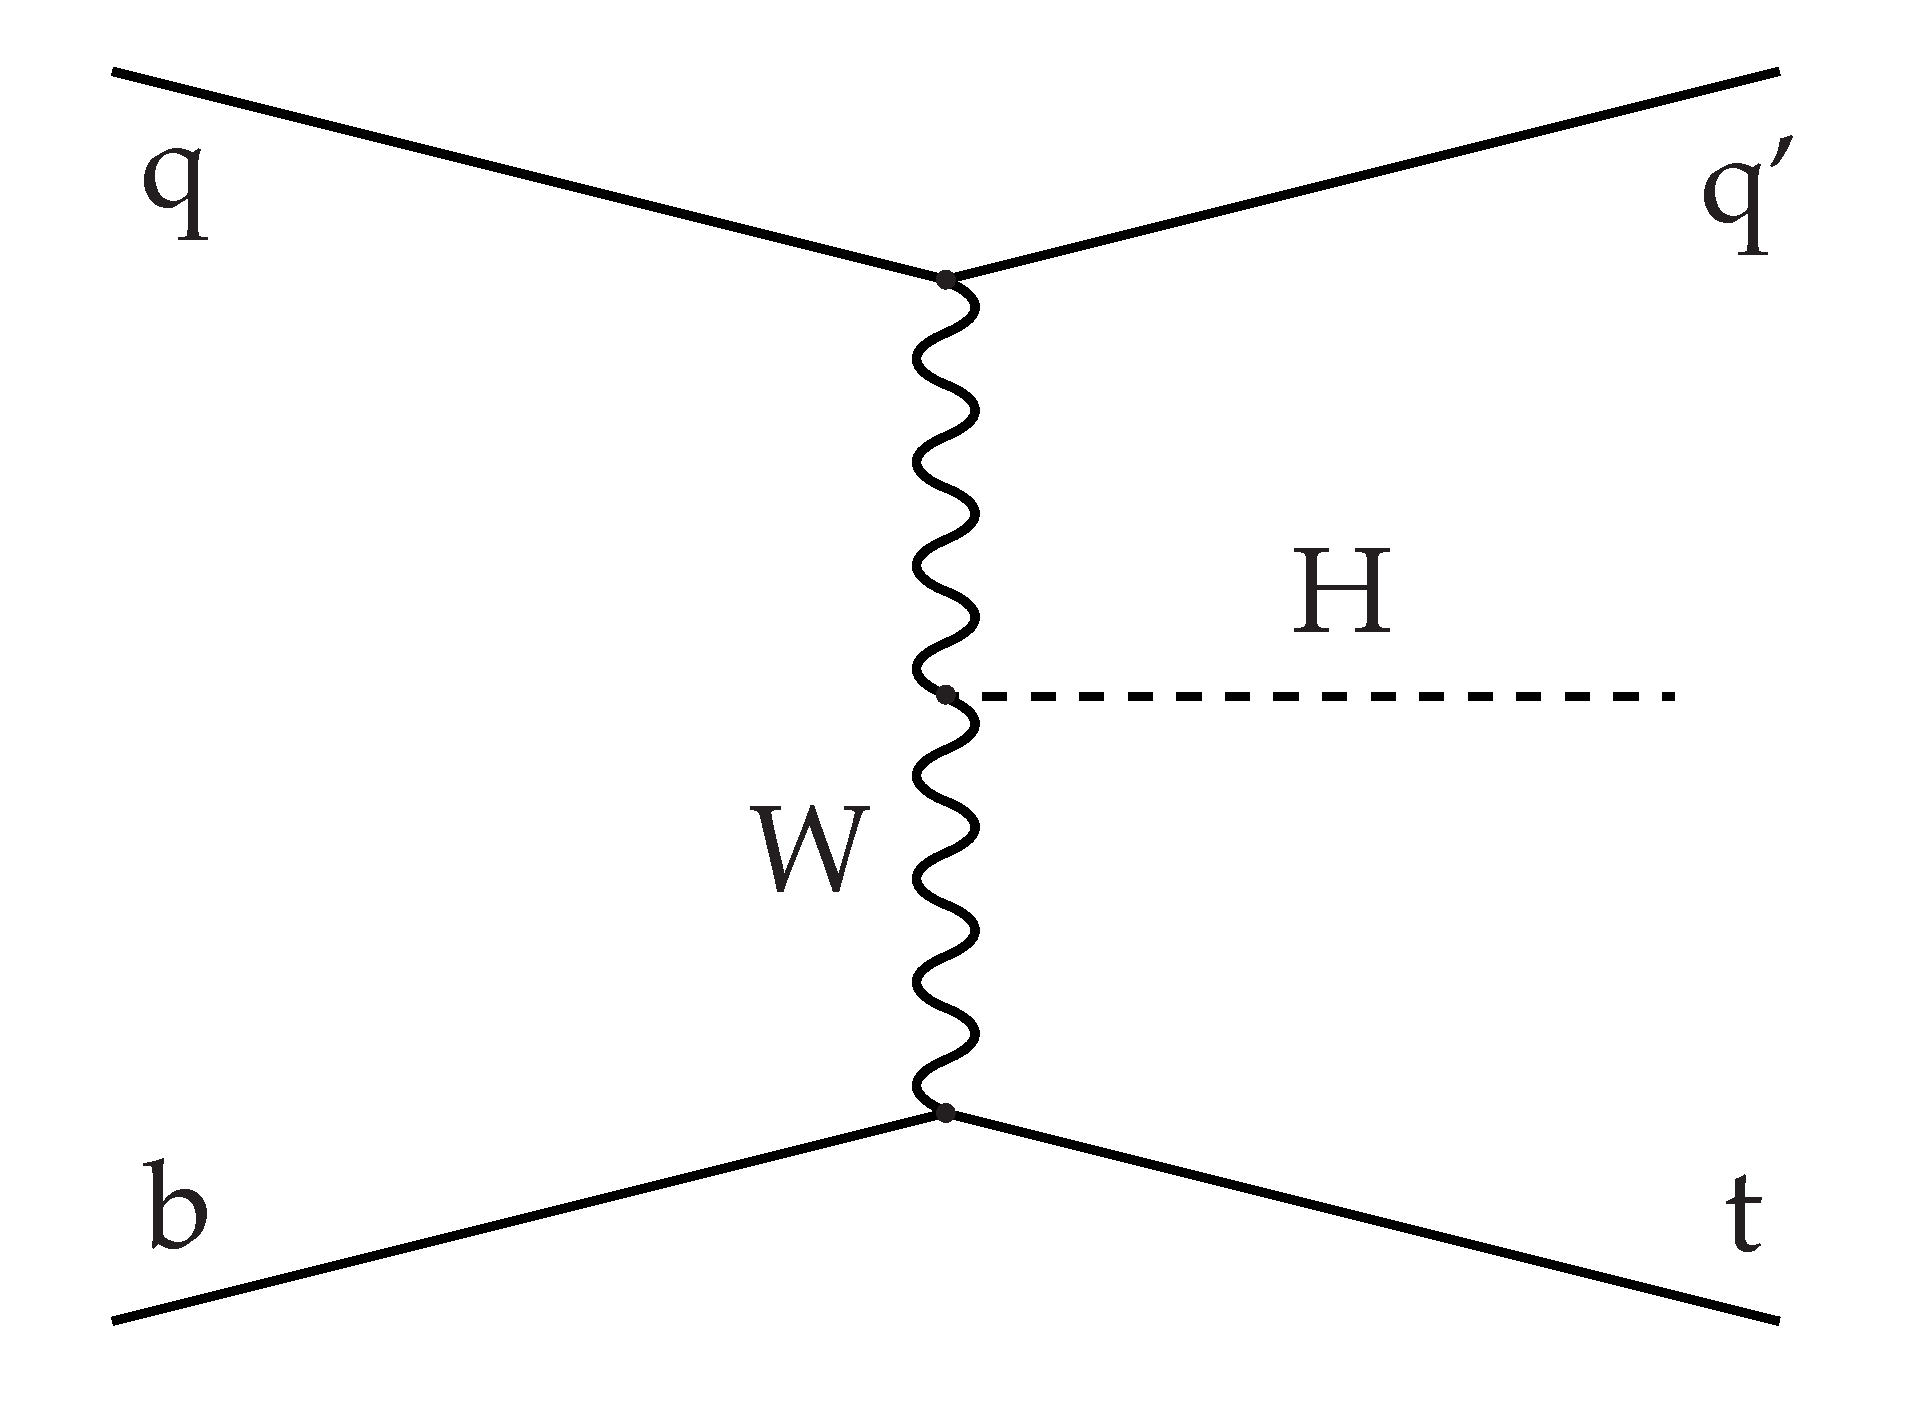
\includegraphics[width=0.3\textwidth]{Figures/feynman_tHq1.pdf}\hspace{1cm}
	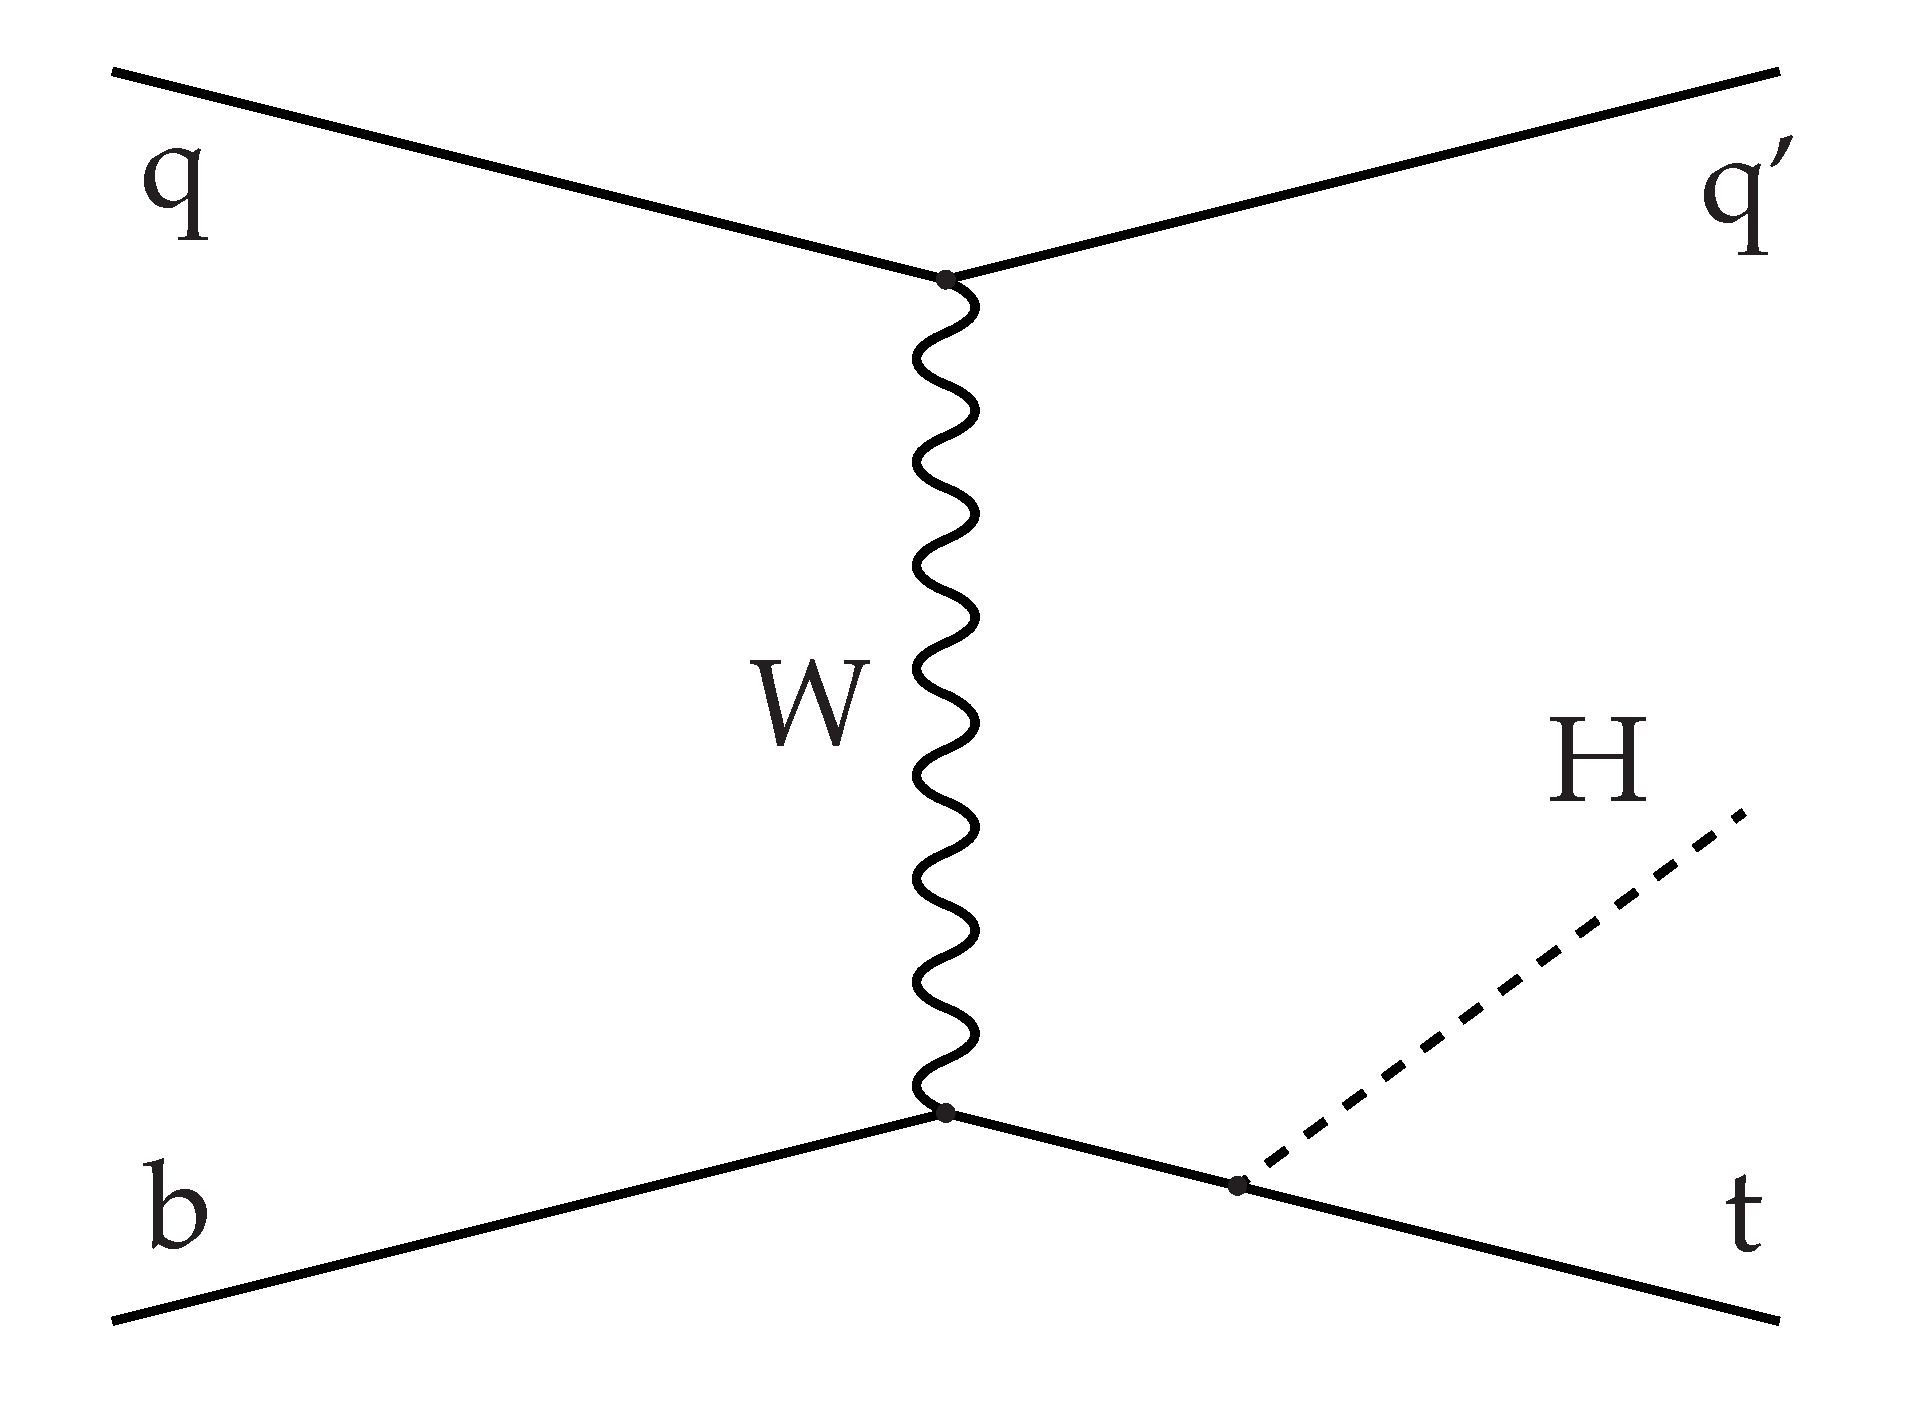
\includegraphics[width=0.3\textwidth]{Figures/feynman_tHq2.pdf}\vspace{.5cm}
	\caption{Dominant leading order Feynman diagrams for the production of \tHq\ events. The Higgs boson is either radiated from the \PW\ boson (left) or the top quark (right).\label{fig:diagrams}}
\end{figure}

% \cite{ennio, Frederix:2009yq, MadGraph5_aMCNLO_2, Frederix:2011ss}, being ten times smaller that the one corresponding to the \ttH production, with an approximate value of 130~fb~\cite{Dittmaier:2011ti,Dittmaier:2012vm,Heinemeyer:2013tqa}.

% Recent work in the literature thus suggested the investigation of \tHq production in the Higgs boson decaying to a pair of photons~\cite{Biswas:2012bd,Biswas:2013xva}, to a pair of b quarks~\cite{ennio}, or Higgs boson decays to leptonic final states~\cite{Biswas:2013xva}.

Direct searches for \tHq\ production using all relevant Higgs decay modes have previously been carried out by CMS in the 8\TeV\ dataset~\cite{thqpaper} and in the 2015 13\TeV\ dataset using the \Hbb\ channel~\cite{CMS-PAS-HIG-16-019}.
In the full 2016 13\TeV\ dataset, a search for \ttH\ production in multilepton final states recently produced first evidence for associated production of top quarks and Higgs bosons~\cite{PAS-HIG-17-004}.

This note reports a search for \tHq\ production in leptonic final states using the full 2016 LHC dataset of at 13\TeV, corresponding to an integrated luminosity of 35.9\fbinv.
Multilepton final states with either two same-sign leptons or three leptons target the case where the Higgs boson decays to a pair of \W bosons, $\tau$ leptons, or \Z\ bosons, and where the top quark decays leptonically.
The results are interpreted as a function of the ratio of two dimensionless modifiers of Higgs couplings: that of the top-Higgs coupling, \Ct, and of the coupling of vector bosons and the Higgs, \CV.
A description of the CMS detector can be found in Ref.~\cite{Chatrchyan:2008zzk}.

The analysis is designed to efficiently identify and select prompt leptons from on-shell \PW\ and \Z\ boson decays and to reject non-prompt leptons from \cPqb\ quark decays and spurious lepton signatures from hadronic jets.
Events are then selected in the various lepton channels, and are required to contain hadronic jets, some of which must be consistent with \cPqb\ quark hadronization.
Finally, the signal yield is extracted by simultaneously fitting the output of two dedicated multivariate discriminants (trained to separate the \tHq\ signal from the two dominant backgrounds) in all categories.

With respect to the 8\TeV\ analysis, the object selections have been adjusted for the updated LHC running conditions at 13\TeV, the lepton identification has been improved, and more powerful multivariate analysis techniques are used for the signal extraction.

